\documentclass[a4paper, 12pt]{article}

\usepackage{listings}
\usepackage{color}
\usepackage{algorithm}
\usepackage{algpseudocode}
\usepackage{amsmath}
\usepackage{graphicx}

\setlength{\parskip}{\baselineskip}%
\setlength{\parindent}{0pt}%

\definecolor{dkgreen}{rgb}{0,0.6,0}
\definecolor{gray}{rgb}{0.5,0.5,0.5}
\definecolor{mauve}{rgb}{0.58,0,0.82}

\definecolor{pred}{rgb}{0.9,0,0}

\definecolor{javared}{rgb}{0.6,0,0} % for strings
\definecolor{javagreen}{rgb}{0.25,0.5,0.35} % comments
\definecolor{javapurple}{rgb}{0.5,0,0.35} % keywords
\definecolor{javadocblue}{rgb}{0.25,0.35,0.75} % javadoc

\lstset{frame=tb,
  language=Java,
  aboveskip=3mm,
  belowskip=3mm,
  showstringspaces=false,
  columns=flexible,
  basicstyle={\small\ttfamily},
  numbers=none,
  numberstyle=\tiny\color{gray},
  keywordstyle=\color{javapurple},
  commentstyle=\color{javagreen},
  stringstyle=\color{blue},
  breaklines=true,
  breakatwhitespace=true,
  tabsize=2,
  basicstyle=\tiny
}


\title{Master Thesis}% \\ \vspace{2 mm} {\large Group 4}}
\author{
    Rusvik, Johan Alexander\\
    \texttt{johan.rusvik@student.uib.no}
}
\date{10.11.2014}

\begin{document}

\maketitle

\newpage
\tableofcontents

\newpage
\listoffigures

%\newpage
%\listoftables

\newpage
\listofalgorithms

\newpage
\section{Introduction}

\subsection{Existing Algorithms}
Chen et al. \cite{Chen} used the Centroid and Weighted Centroid algorithms, amongst others, to examine the positioning accuracy of a GSM beacon-based location system in a metropolitan environment. Yang et al. \cite{Yang} studied the Weighted Centroid and Strongest Received Signal Strength algorithms for cell tower localization.

\subsubsection{Centroid}
The Centroid algorithm estimates a cell tower's position to be the geometric center of the measurements for that cell. It is the mean of the measurements' longitudes and latitudes.

Below follows the mathematical expression for a cell tower's position in a cell with $n$ measurements, where $lon$=longitude and $lat$=latitude, and the pseudocode for the algorithm.
\begin{gather*}
lon_{cellTower} = \frac{1}{n}\sum^{n}_{i=1}\left(lon_i\right), \textnormal{and}\\
lat_{cellTower} = \frac{1}{n}\sum^{n}_{i=1}\left(lat_i\right)
\end{gather*}

\newpage
\begin{algorithm}
\caption{Centroid}
\label{alg:centroid}
\begin{algorithmic}[1]
\Procedure{Centroid}{measurements $\gets$ a list of measurements for a cell}
\State sumOfLongitudes $\gets 0.0$
\State sumOfLatitudes $\gets 0.0$
\For{$\textbf{each}$ m $\in$ measurements}
\State sumOfLongitudes $\gets$ sumOfLongitudes + m.longitude
\State sumOfLatitudes $\gets$ sumOfLatitudes + m.latitude
\EndFor
\State cellTowerLongitude $\gets$ sumOfLongitudes $\div$ measurements.size
\State cellTowerLatitude $\gets$ sumOfLatitudes $\div$ measurements.size
\State \Return cellTowerLongitude, cellTowerLatitude
\EndProcedure
\end{algorithmic}
\end{algorithm}

\subsubsection{Weighted Centroid}
The Weighted Centroid algorithm is an extension of the Centroid algorithm. Here, the measurements are given weights based on the \textit{received signal strength} (RSS) at each measurement. The measurements with strong signals are likely to be closer to the cell tower's real position than those with weaker signals, so we want to emphasize these measurements when calculating the cell tower's position. The unit of measurement for these kind of signals are \textit{Decibel-milliwatts} (dBm) and they range from approximately -30 dBm and lower. Due to the negative values we want to translate them into weights with positive values to make them viable to use for calculations.

Below follows the mathematical expression for a cell tower's position in a cell with $n$ measurements, where $lon$=longitude, $lat$=latitude and $w$ is a measurement's weight based on the RSS, and the pseudocode for the algorithm.
\begin{gather*}
lon_{cellTower} = \frac{1}{\sum^{n}_{j=1}w_j}\sum^{n}_{i=1}\left(lon_i \times w_i\right), \textnormal{and}\\
lat_{cellTower} = \frac{1}{\sum^{n}_{j=1}w_j}\sum^{n}_{i=1}\left(lat_i \times w_i\right)
\end{gather*}

\begin{algorithm}
\caption{Weighted Centroid}
\label{alg:weightedcentroid}
\begin{algorithmic}[1]
\Procedure{WeightedCentroid}{measurements $\gets$ a list of measurements for a cell}
\State sumOfWeights $\gets 0$
\For{$\textbf{each}$ m $\in$ measurements}
\State sumOfWeights $\gets$ sumOfWeights$+$m.signal 
\EndFor
\State x $\gets 0.0$
\State y $\gets 0.0$
\For{$\textbf{each}$ m $\in$ measurements}
\State x $\gets$ x$+($m.longitude$\times$m.signal$)$
\State y $\gets$ y$+($m.latitude$\times$m.signal$)$
\EndFor
\State cellTowerLongitude $\gets$ x $\div$ sumOfWeights
\State cellTowerLatitude $\gets$ y $\div$ sumOfWeights
\State \Return cellTowerLongitude, cellTowerLatitude
\EndProcedure
\end{algorithmic}
\end{algorithm}

\subsubsection{Strongest Received Signal Strength}
The Strongest RSS algorithm estimates a cell tower's position as the position of the measurement with the strongest observed RSS from that cell tower. If multiple measurements qualify, we apply algorithm \ref{alg:centroid} on these.

Below follows the mathematical expression for a cell tower's position in a cell with $n$ measurements, where $lon$=longitude, $lat$=latitude and $w$ is a measurement's weight based on the RSS, and the pseudocode for the algorithm.
%\begin{equation}
%\begin{align*}
\begin{gather*}
lon_{cellTower}=\frac{1}{m}\sum^{m}_{i=1}\left(lon_i\right), \textnormal{ and}\\ 
lat_{cellTower}=\frac{1}{m}\sum^{m}_{i=1}\left(lat_i\right), \textnormal{ where}\\ 
%w_j = max(w_1,w_2,...,w_n), \textnormal{ and}\\ 
m = |W| = \{w:w\in max(w_1,w_2,...,w_n)\}
\end{gather*}
%\textnormal{ is the cardinality of the set }
%\end{align*}
%\end{equation}
\begin{algorithm}
\caption{Strongest Received Signal Strength}
\label{alg:strongestrss}
\begin{algorithmic}[1]
\Procedure{StrongestRSS}{measurements $\gets$ a list of measurements for a cell}
\State strongestSignalMeasurements $\gets$ a list to store the measurements with the strongest signal
\State currentStrongestSignal $\gets -1$
\For{$\textbf{each}$ m $\in$ measurements}
\If{m.signal $>$ currentStrongestSignal}
\State \textbf{clear} strongestSignalMeasurements
\State \textbf{add} m \textbf{to} strongestSignalMeasurements
\State currentStrongestSignal $\gets$ m.signal
\ElsIf{m.signal $=$ currentStrongestSignal}
\State \textbf{add} m \textbf{to} strongestSignalMeasurements
\EndIf
\EndFor
\State x $\gets 0.0$
\State y $\gets 0.0$
\For{$\textbf{each}$ m $\in$ strongestSignalMeasurements}
\State x $\gets$ x + m.longitude
\State y $\gets$ y + m.latitude
\EndFor
\State cellTowerLongitude $\gets$ x $\div$ strongestSignalMeasurements.size
\State cellTowerLatitude $\gets$ y $\div$ strongestSignalMeasurements.size
\State \Return cellTowerLongitude, cellTowerLatitude
\EndProcedure
\end{algorithmic}
\end{algorithm}

\newpage
\subsection{Testdata}
We wrote a small Java program for generating testdata. Below follow three example screenshots where we apply algorithm \ref{alg:centroid}, \ref{alg:weightedcentroid} and \ref{alg:strongestrss} on three random generated cells with 10, 20 and 40 measurements, respectively. The cell tower is placed in the middle and the measurements are generated randomly around it.
\begin{itemize}
\item \text{Black circles:} Measurements
\item \text{Black square:} Real position of cell tower
\item \text{Blue square:} Position of cell tower calculated by Centroid
\item \text{Green square:} Position of cell tower calculated by Weighted Centroid
\item \text{Red square:} Position of cell tower calculated by Strongest RSS
\end{itemize}

\begin{figure}[h!]
\label{fig:10meas}
  \centering
  %\begin{subfigure}[t]{0.45\textwidth}
    %\centering
    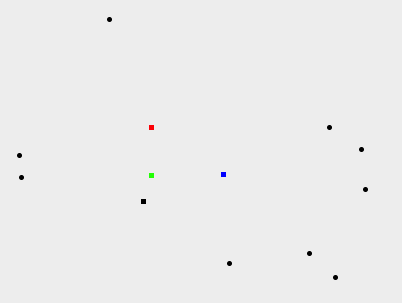
\includegraphics[scale=0.8]{testData_10meas.png}
    \caption{Random generated cell with 10 measurements}
  %\end{subfigure}
  %\hspace{.03\textwidth}
  %\begin{subfigure}[t]{0.45\textwidth}
    %\centering
    %\includegraphics[width=10em]{Steiner_after.png}
    %\caption{\textsf{Grapher} with Steiner tree highlighted}
  %\end{subfigure}
  %\caption{\textsf{Grapher} before and after computing the Steiner tree.}
\end{figure}

\newpage
\begin{figure}[h!]
\label{fig:20meas}
\centering
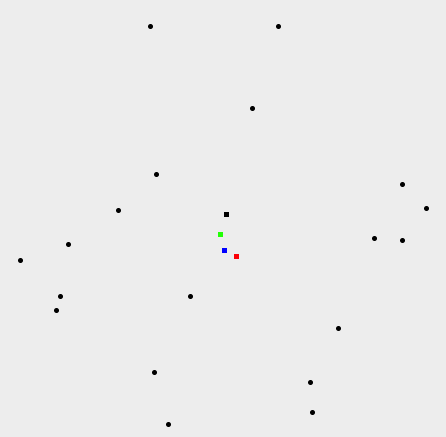
\includegraphics[scale=0.56]{testData_20meas.png}
\caption{Random generated cell with 20 measurements}
\end{figure}

\begin{figure}[h!]
\label{fig:40meas}
\centering
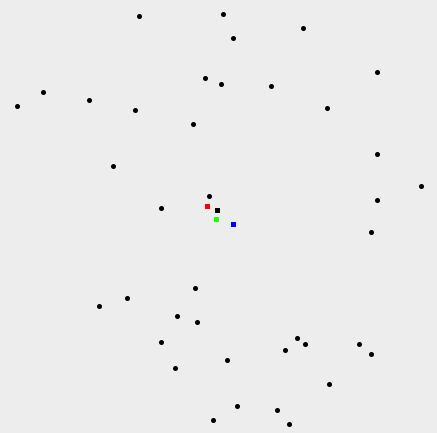
\includegraphics[scale=0.56]{testData_40meas.png}
\caption{Random generated cell with 40 measurements}
\end{figure}


%\newpage
%\section{Work}

%\subsection{Centroid}


%\newpage
%\subsection{Weighted Centroid}



%\newpage
%\subsection{Strongest Received Signal Strength}



%\section{Conclusion}


\newpage
\bibliographystyle{abbrv}
\bibliography{references}

\newpage
\appendix
\section{Code}
\label{app:code}
\begin{lstlisting}
package testdata;

import java.awt.geom.Point2D;
import java.util.Random;

public class Measurement {
	
	private Point2D.Double coordinates;
	
	// Signal Strength = sqrt((x2-x1)^2 + (y2-y1)^2) multiplied by -1 to achieve realistic dBm
	private int signalStrength;
	
	// Weight = 113 - (-1 * Signal Strength)
	private int weight;
	
	public Measurement(double longitude, double latitude) {
		this.coordinates = new Point2D.Double(longitude, latitude);
		this.signalStrength = 99;
		this.weight = -99;
	}

	public Point2D.Double getCoordinates() {
		return coordinates;
	}

	public void setCoordinates(Point2D.Double coordinates) {
		this.coordinates = coordinates;
	}

	public int getSignalStrength() {
		return signalStrength;
	}

	public void setSignalStrength(int signalStrength) {
		this.signalStrength = signalStrength;
	}

	public int getWeight() {
		return weight;
	}

	public void setWeight(int weight) {
		this.weight = weight;
	}

	@Override
	public String toString() {
		String s = String.format("Measurement coordinates: [%.1f,%.1f] - Signal Strength: %d dBm - Weight: %d", 
				this.coordinates.x, this.coordinates.y, this.signalStrength, this.weight);
		return s;
	}

	public static Measurement generateRandomMeasurement(int maxX, int maxY) {
		double x = (double) new Random().nextInt(maxX+1);
		double y = (double) new Random().nextInt(maxY+1);
		
		return new Measurement(x, y);
	}
}

package testdata;

import java.awt.geom.Point2D;
import java.util.ArrayList;
import java.util.List;

public class Cell {
	
	protected static final String MEASUREMENTS_ALL = "all measurements";
	protected static final String MEASUREMENTS_THRESHOLD = "measurements filtered";
	
	protected static final int CELL_X_Y_VALUE = 113;
	protected static final int MEASUREMENT_X_Y_LIMIT = 226;
	
	private Point2D.Double cellTowerCoordinates;
	
	// Pointer
	private List<Measurement> measurements;
	
	// List for storing all measurements
	private List<Measurement> measurementsAll;
	
	// List for storing measurements above a certain weight threshold
	private List<Measurement> measurementsWithThreshold;
	
	public Cell() {
		this.cellTowerCoordinates = new Point2D.Double((double) CELL_X_Y_VALUE, (double) CELL_X_Y_VALUE);
		this.measurementsAll = new ArrayList<Measurement>();
		this.measurementsWithThreshold = new ArrayList<Measurement>();
	}

	public Point2D.Double getCellTowerCoordinates() {
		return cellTowerCoordinates;
	}

	public void setCellTowerCoordinates(Point2D.Double cellTowerCoordinates) {
		this.cellTowerCoordinates = cellTowerCoordinates;
	}

	public List<Measurement> getMeasurements() {
		return measurements;
	}

	public void setMeasurements(List<Measurement> measurements) {
		this.measurements = measurements;
	}

	public void addRandomMeasurements(int measurements, int maxX, int maxY) {
		
		for(int i = 0; i < measurements; i++) {

			Measurement measurement;
			double d;
			do {
				measurement = Measurement.generateRandomMeasurement(maxX, maxY);
				d = this.cellTowerCoordinates.distance(measurement.getCoordinates());
				
			} while(d > 113.0);
			
			int dBm = Surface.doubleToInt(d)*-1;
			measurement.setSignalStrength(dBm);
			
			int weight = 113 - (-1*measurement.getSignalStrength());
			measurement.setWeight(weight);
		
			this.measurementsAll.add(measurement);
			
			this.useMeasurements(MEASUREMENTS_ALL);
		}
		return;
	}
	
	protected Cell applyWeightThreshold(int minimumWeight) {
		this.measurementsWithThreshold.clear();
		for(Measurement measurement : this.measurementsAll) {
			if(measurement.getWeight() >= minimumWeight) {
				this.measurementsWithThreshold.add(measurement);
			}
		}
		return this;
	}
	
	protected Cell useMeasurements(String measurementsList) {
		if(measurementsList.equals(MEASUREMENTS_ALL)) {
			this.measurements = this.measurementsAll;
		}
		else if(measurementsList.equals(MEASUREMENTS_THRESHOLD)) {
			this.measurements = this.measurementsWithThreshold;
		}
		else {
			throw new IllegalArgumentException("There is no such list");
		}
		return this;
	}
	
	@Override
	public String toString() {
		String s = String.format("Cell Tower Coordinates: [%.1f,%.1f]\n\tMeasurements: %d", 
				this.cellTowerCoordinates.x, this.cellTowerCoordinates.y, this.measurements.size());
		for(Measurement measurement : this.measurements) {
			s += "\n\t"+measurement.toString();
		}
		s += "\n";
		return s;
	}

	public static Cell generateCellWithRandomMeasurements(int measurements) {
		
		Cell cell = new Cell();
		
		if(measurements > 0) {
			cell.addRandomMeasurements(measurements, MEASUREMENT_X_Y_LIMIT, MEASUREMENT_X_Y_LIMIT);
		}
				
		return cell;
	}
}

package testdata;

import java.awt.geom.Point2D;
import java.util.ArrayList;
import java.util.List;

public class Statistics {
	
	private Cell cell;
	
	private Point2D.Double centroidCoordinates;
	private Point2D.Double weightedCentroidCoordinates;
	private Point2D.Double strongestRSSCoordinates;
	
	private Point2D.Double centroidWithThresholdCoordinates;
	private Point2D.Double weightedCentroidWithThresholdCoordinates;
	private Point2D.Double strongestRSSWithThresholdCoordinates;
	
	
	public Statistics(int measurements) {
		this.cell = Cell.generateCellWithRandomMeasurements(measurements);
		this.centroidCoordinates = centroid(this.cell);
		this.weightedCentroidCoordinates = weightedCentroid(this.cell);
		this.strongestRSSCoordinates = strongestRSS(this.cell);
		
		int threshold = 50;
		
		this.centroidWithThresholdCoordinates = centroid(this.cell.applyWeightThreshold(threshold).useMeasurements(Cell.MEASUREMENTS_THRESHOLD));
		this.weightedCentroidWithThresholdCoordinates = weightedCentroid(this.cell);
		this.strongestRSSWithThresholdCoordinates = strongestRSS(this.cell);	
		
		System.out.println(this.toString());
	}

	public static void main(String[] args) {
		
		Statistics statistics = new Statistics(5);

		System.out.println("\nEND OF PROGRAM");
	}
	
	public Cell getCell() {
		return cell;
	}

	public void setCell(Cell cell) {
		this.cell = cell;
	}

	public Point2D.Double getCentroidCoordinates() {
		return centroidCoordinates;
	}

	public void setCentroidCoordinates(Point2D.Double centroidCoordinates) {
		this.centroidCoordinates = centroidCoordinates;
	}

	public Point2D.Double getWeightedCentroidCoordinates() {
		return weightedCentroidCoordinates;
	}

	public void setWeightedCentroidCoordinates(
			Point2D.Double weightedCentroidCoordinates) {
		this.weightedCentroidCoordinates = weightedCentroidCoordinates;
	}

	public Point2D.Double getStrongestRSSCoordinates() {
		return strongestRSSCoordinates;
	}

	public void setStrongestRSSCoordinates(Point2D.Double strongestRSSCoordinates) {
		this.strongestRSSCoordinates = strongestRSSCoordinates;
	}
	
	
	public Point2D.Double getCentroidWithThresholdCoordinates() {
		return centroidWithThresholdCoordinates;
	}

	public void setCentroidWithThresholdCoordinates(
			Point2D.Double centroidWithThresholdCoordinates) {
		this.centroidWithThresholdCoordinates = centroidWithThresholdCoordinates;
	}

	public Point2D.Double getWeightedCentroidWithThresholdCoordinates() {
		return weightedCentroidWithThresholdCoordinates;
	}

	public void setWeightedCentroidWithThresholdCoordinates(
			Point2D.Double weightedCentroidWithThresholdCoordinates) {
		this.weightedCentroidWithThresholdCoordinates = weightedCentroidWithThresholdCoordinates;
	}

	public Point2D.Double getStrongestRSSWithThresholdCoordinates() {
		return strongestRSSWithThresholdCoordinates;
	}

	public void setStrongestRSSWithThresholdCoordinates(
			Point2D.Double strongestRSSWithThresholdCoordinates) {
		this.strongestRSSWithThresholdCoordinates = strongestRSSWithThresholdCoordinates;
	}

	@Override
	public String toString() {
		String s = "";
		if(this.cell.useMeasurements(Cell.MEASUREMENTS_ALL).getMeasurements().size() <= 5) {
			s += this.cell.useMeasurements(Cell.MEASUREMENTS_ALL).toString();
			s += "\n";
		}
		
		s += "\t\t\tCell Tower Longitude\tCell Tower Latitude\tError\n";
		s += String.format("Real\t\t\t%.1f\t\t\t%.1f\t\t\t%.1f\n", this.cell.getCellTowerCoordinates().getX(), this.cell.getCellTowerCoordinates().getY(), this.cell.getCellTowerCoordinates().distance(this.cell.getCellTowerCoordinates()));
		s += String.format("Centroid\t\t%.1f\t\t\t%.1f\t\t\t%.1f\n", this.centroidCoordinates.getX(), this.centroidCoordinates.getY(), this.cell.getCellTowerCoordinates().distance(this.getCentroidCoordinates()));
		s += String.format("Centroid >= 50\t\t%.1f\t\t\t%.1f\t\t\t%.1f\n",this.centroidWithThresholdCoordinates.getX(), this.centroidWithThresholdCoordinates.getY(), this.cell.getCellTowerCoordinates().distance(this.getCentroidWithThresholdCoordinates()));
		s += String.format("Weighted Centroid\t%.1f\t\t\t%.1f\t\t\t%.1f\n", this.weightedCentroidCoordinates.getX(), this.weightedCentroidCoordinates.getY(), this.cell.getCellTowerCoordinates().distance(this.getWeightedCentroidCoordinates()));
		s += String.format("Weighted Centroid >= 50\t%.1f\t\t\t%.1f\t\t\t%.1f\n",this.weightedCentroidWithThresholdCoordinates.getX(), this.weightedCentroidWithThresholdCoordinates.getY(), this.cell.getCellTowerCoordinates().distance(this.getWeightedCentroidWithThresholdCoordinates()));
		s += String.format("Strongest RSS\t\t%.1f\t\t\t%.1f\t\t\t%.1f\n", strongestRSSCoordinates.getX(), strongestRSSCoordinates.getY(), this.cell.getCellTowerCoordinates().distance(this.getStrongestRSSCoordinates()));
		s += String.format("Strongest RSS >= 50\t%.1f\t\t\t%.1f\t\t\t%.1f\n",this.strongestRSSWithThresholdCoordinates.getX(), this.strongestRSSWithThresholdCoordinates.getY(), this.cell.getCellTowerCoordinates().distance(this.getStrongestRSSWithThresholdCoordinates()));

		return s;
	}
	
	private static Point2D.Double weightedCentroid(Cell cell) {
		
		int sumOfWeights = 0;
		for(Measurement measurement : cell.getMeasurements()) {
			sumOfWeights += measurement.getWeight();
		}
				
		double cellTowerLongitude = 0.0;
		double cellTowerLatitude = 0.0;
		for(Measurement measurement : cell.getMeasurements()) {
			double weightRatio = measurement.getWeight()/(double)sumOfWeights;

			cellTowerLongitude += (measurement.getCoordinates().getX()*weightRatio);
			cellTowerLatitude += (measurement.getCoordinates().getY()*weightRatio);
		}
		return new Point2D.Double(cellTowerLongitude, cellTowerLatitude);
	}
	
	private static Point2D.Double centroid(Cell cell) {
		double sumOfLongitudes = 0;
		double sumOfLatitudes = 0;
		for(Measurement measurement : cell.getMeasurements()) {
			sumOfLongitudes += measurement.getCoordinates().getX();
			sumOfLatitudes += measurement.getCoordinates().getY();
		}
		double cellTowerLongitude = sumOfLongitudes/cell.getMeasurements().size();
		double cellTowerLatitude = sumOfLatitudes/cell.getMeasurements().size();
		
		return new Point2D.Double(cellTowerLongitude, cellTowerLatitude);
	}
	
	private static Point2D.Double strongestRSS(Cell cell) {
		int currentStrongestWeight = -1;
		List<Measurement> strongestWeightMeasurements = new ArrayList<Measurement>();
		for(Measurement measurement : cell.getMeasurements()) {
			if(measurement.getWeight() > currentStrongestWeight) {
				strongestWeightMeasurements.clear();
				strongestWeightMeasurements.add(measurement);
				currentStrongestWeight = measurement.getWeight();
			}
			else if(measurement.getWeight() == currentStrongestWeight) {
				strongestWeightMeasurements.add(measurement);
			}
		}
		double sumOfLongitudes = 0.0;
		double sumOfLatitudes = 0.0;
		for(Measurement measurement : strongestWeightMeasurements) {
			sumOfLongitudes += measurement.getCoordinates().getX();
			sumOfLatitudes += measurement.getCoordinates().getY();
		}
		double cellTowerLongitude = sumOfLongitudes/strongestWeightMeasurements.size();
		double cellTowerLatitude = sumOfLatitudes/strongestWeightMeasurements.size();
		return new Point2D.Double(cellTowerLongitude, cellTowerLatitude);
	}
}

package testdata;

import java.awt.Color;
import java.awt.Dimension;
import java.awt.EventQueue;
import java.awt.Graphics;
import java.awt.Graphics2D;
import java.awt.Insets;
import java.awt.RenderingHints;
import java.awt.geom.AffineTransform;
import java.awt.geom.Point2D;
import java.util.List;

import javax.swing.JFrame;
import javax.swing.JPanel;

class Surface extends JPanel {
	
	Statistics statistics;
	
	public Surface() {
		this.statistics = new Statistics(40);
	}
	
	private void doDrawing(Graphics g) {
		Graphics2D g2d = (Graphics2D) g;
		
//		AffineTransform transform = AffineTransform.getTranslateInstance(0, 700);
//		transform.scale(700, -700);
//		g2d.setTransform(transform);
		
		g2d.setColor(Color.black);
		
		RenderingHints rh = new RenderingHints(RenderingHints.KEY_ANTIALIASING,
				RenderingHints.VALUE_ANTIALIAS_ON);
		rh.put(RenderingHints.KEY_RENDERING, RenderingHints.VALUE_RENDER_QUALITY);
		g2d.setRenderingHints(rh);
		
		Dimension size = getSize();
		Insets insets = getInsets();
		int w = size.width - insets.left - insets.right;
		int h = size.height - insets.top - insets.bottom;
		
		// Cell Tower real coords
		Point2D.Double cellTower = this.statistics.getCell().getCellTowerCoordinates();
		int x = doubleToInt(enlarge(cellTower.getX()));
		int y = invertLatitude(h, enlarge(cellTower.getY()));
		g2d.fillRect(x, y, 5, 5);
		
		// Measurements coords
		List<Measurement> measurements = this.statistics.getCell().getMeasurements();
		for(Measurement measurement : measurements) {
			x = doubleToInt(enlarge(measurement.getCoordinates().getX()));
			y = invertLatitude(h, enlarge(measurement.getCoordinates().getY()));
			g2d.fillOval(x, y, 5, 5);
		}
		
		// Cell Tower Centroid coords
		g2d.setColor(Color.blue);
		Point2D.Double centroidCoordinates = this.statistics.getCentroidCoordinates();
		x = doubleToInt(enlarge(centroidCoordinates.getX()));
		y = invertLatitude(h, enlarge(centroidCoordinates.getY()));
		g2d.fillRect(x, y, 5, 5);
		
		// Cell Tower Weighted Centroid coords
		g2d.setColor(Color.green);
		Point2D.Double weightedCentroidCoordinates = this.statistics.getWeightedCentroidCoordinates();
		x = doubleToInt(enlarge(weightedCentroidCoordinates.getX()));
		y = invertLatitude(h, enlarge(weightedCentroidCoordinates.getY()));
		g2d.fillRect(x, y, 5, 5);
		
		// Cell Tower Strongest RSS coords
		g2d.setColor(Color.red);
		Point2D.Double strongestRSSCoordinates = this.statistics.getStrongestRSSCoordinates();
		x = doubleToInt(enlarge(strongestRSSCoordinates.getX()));
		y = invertLatitude(h, enlarge(strongestRSSCoordinates.getY()));
		g2d.fillRect(x, y, 5, 5);
		
		// Cell Tower Centroid with threshold coords
		g2d.setColor(Color.cyan);
		Point2D.Double centroidWithThresholdCoordinates = this.statistics.getCentroidWithThresholdCoordinates();
		x = doubleToInt(enlarge(centroidWithThresholdCoordinates.getX()));
		y = invertLatitude(h, enlarge(centroidWithThresholdCoordinates.getY()));
		g2d.fillRect(x, y, 5, 5);
		
		// Cell Tower Weighted Centroid with threshold coords
		g2d.setColor(Color.orange);
		Point2D.Double weightedCentroidWithThresholdCoordinates = this.statistics.getWeightedCentroidWithThresholdCoordinates();
		x = doubleToInt(enlarge(weightedCentroidWithThresholdCoordinates.getX()));
		y = invertLatitude(h, enlarge(weightedCentroidWithThresholdCoordinates.getY()));
		g2d.fillRect(x, y, 5, 5);
		
		// Cell Tower Strongest RSS with threshold coords
		g2d.setColor(Color.pink);
		Point2D.Double strongestRSSWithThresholdCoordinates = this.statistics.getStrongestRSSWithThresholdCoordinates();
		x = doubleToInt(enlarge(strongestRSSWithThresholdCoordinates.getX()));
		y = invertLatitude(h, enlarge(strongestRSSWithThresholdCoordinates.getY()));
		g2d.fillRect(x, y, 5, 5);
	}
	
	protected static int invertLatitude(int height, double latitude) {
		double newY = ((double)height - latitude);
		return doubleToInt(newY);
	}
	
	protected static int doubleToInt(double d) {
		int toInt = (int)d;
		if(d-(double)toInt >= 0.5) {
			return toInt+1;
		}
		else
			return toInt;
	}
	
	private double enlarge(double d) {
		return d*2;
	}
	
	@Override
	public void paintComponent(Graphics g) {
		super.paintComponent(g);
		doDrawing(g);
	}
}

public class Map extends JFrame {
	
	final static int WIDTH = 700;
	final static int HEIGHT = 700;
	
	public Map() {
		initUI();
	}

	private void initUI() {
		setTitle("Map");
		
		add(new Surface());
		
		setSize(WIDTH, HEIGHT);
		setLocationRelativeTo(null);
		setDefaultCloseOperation(EXIT_ON_CLOSE);
		
	}

	public static void main(String[] args) {
		
		EventQueue.invokeLater(new Runnable() {
			@Override
			public void run() {
				Map map = new Map();
				map.setVisible(true);
			}
		});
	}
}
\end{lstlisting}




































\end{document}